\documentclass[12pt]{article}
\usepackage[portuguese]{babel}
\usepackage[utf8]{inputenc}
\usepackage{graphicx}

\title{Relatório do Projeto de MAC0218 \\ (Parte I)}

\author
{
	Lucas Henrique Bahr Yau \\
	Victor Seiji Hariki\\
	André Luiz Akabane Solak\\
	Gabriely Rangel
}

\date{}

\begin{document}
	\maketitle
	
	\section*{O que foi feito}
	Nesta primeira parte do projeto, focamos na modelagem e implementação do banco de dados e na autenticação do usuário na aplicação.\\
	
	\subsection*{Modelo do banco de dados}
	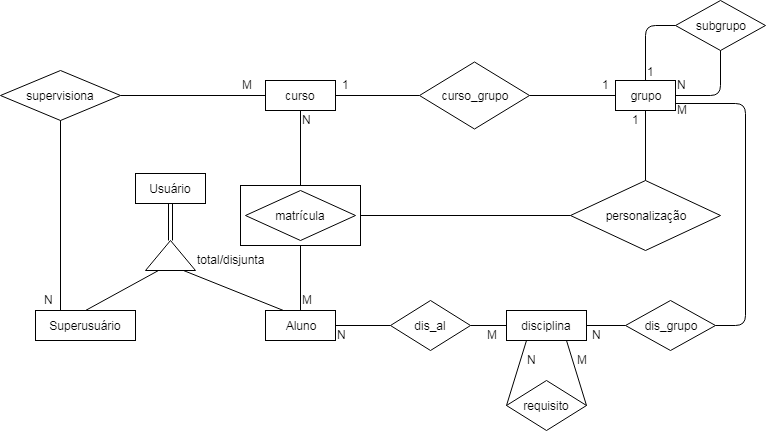
\includegraphics[scale=0.5]{tec}
	
	\section*{Próximos passos}
	\begin{itemize}
	\item Com o banco de dados funcionando, nosso próximo objetivo será implementar os controladores.
	\item Posteriormente, assim que a aplicação possuir uma estrutura mais completa, pretendemos melhorar a visualização do site.
	\end{itemize}
	
	\section*{Dificuldades encontradas}
	\begin{itemize} 
	\item Tivemos várias reuniões para decidir quais dados seriam utilizados/coletados do usuário, e como associamos cada um desses dados. A modelagem pode haver modificações, conforme avançamos no projeto.\\
	\item Sendo esta a primeira vez que desenvolvemos um aplicativo com Rails, tivemos que aprender suas peculiaridades, como o tratamento do modelo "MVC" e seus comandos.
	\end{itemize}
	
	
\end{document}